\documentclass[a4, oneside, 10pt, nobib]{memoir}

%% IMPORTS
% Clickable ref
\usepackage{hyperref}
\usepackage{setspace}
\usepackage{wrapfig}
\usepackage{graphicx}
\usepackage{lipsum}
 \usepackage{soul}

\usepackage{subcaption}

\usepackage{float}

\usepackage{calc}  
\usepackage{enumitem}

\usepackage{xcolor}
\usepackage{minted}
\usepackage[backend=biber, style=numeric, defernumbers]{biblatex}

%% SET THINGS UP
% Add bibliography database
\addbibresource{bibliography.bib}

\definecolor{friendlybg}{HTML}{F8F8F8}

% Minted macros
% Will append "code" to the environment name by default
\newminted{python}{style=friendly, bgcolor=friendlybg, breaklines, tabsize=2}
\newminted{text}{style=friendly, bgcolor=friendlybg, breaklines, tabsize=2, breakanywhere}
\newminted{shell}{style=friendly, bgcolor=friendlybg, breaklines, tabsize=2, breakanywhere}
\newminted{yaml}{style=friendly, bgcolor=friendlybg, breaklines, tabsize=2, breakanywhere}
\newminted{nginx}{style=friendly, bgcolor=friendlybg, breaklines, tabsize=2, breakanywhere}
\newminted{json}{style=friendly, bgcolor=friendlybg, breaklines, tabsize=2, breakanywhere}


\usepackage{tikz}
\usetikzlibrary{positioning}

\tikzset{basic/.style={draw,fill=blue!20,text width=1em,text badly centered}}
\tikzset{input/.style={basic,circle}}
\tikzset{weights/.style={basic,rectangle}}
\tikzset{functions/.style={basic,circle,fill=blue!10}}


% Tables
\usepackage{multirow}

% micro sign != MU
\usepackage{siunitx}

% Typography
\usepackage{fontspec}
	% Numbers={OldStyle,Proportional},Ligatures=TeX
	\setmainfont[]{Minion Pro}
	\setmonofont[Scale=0.85]{Iosevka}
	%\newfontfamily\bold{Tiempos Headline Medium}

 \newcommand{\mcode}[1]{%
  \sethlcolor{friendlybg}{%
  \texttt{\hl{\mbox{#1}}}}%
}

% Captions
\usepackage[font=normalsize, labelfont=bf]{caption}
\captionsetup[table]{position=below}
\captionsetup[figure]{position=below}

% Figures
\graphicspath{ {figures/} }
%\definecolor{gray75}{gray}{0.75}

% Set Table of Contents depth
\setsecnumdepth{subsection}
\settocdepth{subsection}

% Style Abstract (and Acknowledgements)
\renewcommand{\abstractnamefont}{\normalfont\huge\bfseries}
\renewcommand{\abstracttextfont}{\normalfont\normalsize}

% Utilities
\newcommand{\code}{\texttt}

%\settypeblocksize{20cm}{16.5cm}{*}%

\usepackage[nopostdot,style=alttree,nonumberlist,toc]{glossaries}
\glssetwidest{L1 Triggerrr}
\makeglossaries

\newglossaryentry{cms}
{
    name=CMS,
    description={Compact Muon Solenoid detector}
}

\newglossaryentry{dqm}
{
    name=DQM,
    description={Data Quality Monitoring}
}

\newglossaryentry{daq}
{
    name=DAQ,
    description={Data AcQuisition}
}

\newglossaryentry{cern}
{
    name=CERN,
    description={European Organization for Nuclear Research}
}

\newglossaryentry{ls}
{
    name=LS,
    description={LumiSection}
}

\newglossaryentry{lhc}
{
    name=LHC,
    description={Large Hadron Collider}
}


\newglossaryentry{p5}
{
    name=P5,
    description={Point 5 of the LHC, in Cessy (France), home to the CMS detector}
}

\newglossaryentry{lxplus}
{
    name=LXPLUS,
    description={CERN IT Service offering access to Linux machines over SSH}
}

\newglossaryentry{l1}
{
    name=L1 Trigger,
    description={Level 1 Trigger}
}

\newglossaryentry{hlt}
{
    name=HLT,
    description={High Level Trigger}
}

\newglossaryentry{pu}
{
    name=PU,
    description={Pile-up}
}

\newglossaryentry{omds}
{
    name=OMDS,
    description={Online Master Database System, the online master database located at P5 on the CMS online network}
}

\newglossaryentry{OMS}
{
    name=OMS,
    description={CMS Online Monitoring System}
}

\newglossaryentry{WBM}
{
    name=WBM,
    description={CMS Web Based Monitoring}
}




%% DOCUMENT
\begin{document}

% Add revision data
\input{revision}

%\setlrmarginsandblock{2.5cm}{2.5cm}{*}
%\setulmarginsandblock{2.5cm}{*}{1}
%\checkandfixthelayout 

% Frontmatter part is numbered with Romans
\frontmatter

% Preamble:
%  Front, Dedication, Abstract and Acknowledgements
% Based on https://github.com/dubvulture/thesis/blob/master/frontispiece.tex

\thispagestyle{empty}

\begin{wrapfigure}{l}[22mm]{0.20\textwidth}
	\vspace*{-8mm}
	\centering
	
\includegraphics[width=0.20\textwidth]{logo-bicocca.jpg}
\end{wrapfigure}
\large \noindent \textsc{Università degli Studi di Milano Bicocca} \\
\textbf{Dipartimento di Informatica, Sistemistica e Comunicazione \\
	Corso di Laurea Magistrale in Informatica}

\vfill


\begin{center}
	{\Huge \textbf{Experimental Anomaly Detection on CERN CMS Trigger Rates}}
\end{center}

\vfill

\begin{flushleft}
	{\Large \textbf{Supervisor:} \textit{Fabio Stella} \\
		\textbf{Co-supervisor:} \textit{Simone Gennai} \\
		\textbf{Co-supervisor:} \textit{Glenn Dirkx}}
\end{flushleft}

\vspace{8mm}
\par

\begin{flushright}
	{\Large \textbf{Master Thesis} \\
		\textit{Antonio Vivace} \\ 793509}
\end{flushright}

\vfill
\par

\begin{center}
	{\large Academic Year 2019 -- 2020}

	% Print revision data and WIP notice
	\hfill\linebreak
	Work In Progress Draft (!)

	Revision \texttt{\revision} (\texttt{\revisiondate})

	\url{https://avivace.com/thesis.pdf} for the latest build.
\end{center}

\clearpage
\clearpage
\begin{flushright}
	\thispagestyle{empty}
	\vspace*{50 mm}
	To \textit{Meni}, the scientist of the family.

\end{flushright}
\clearpage
\phantomsection
\addcontentsline{toc}{chapter}{Abstract}

\begin{vplace}[0.7]
	\renewcommand*\abstractname{Abstract}

	\begin{abstract}

		\fontsize{11}{12}\selectfont\baselineskip=1.2em

		High Energy Physics experiments involve large amount of complex systems subject to anomalies and malfunctioning. They generate a lot of high dimensional and contextual data that must be monitored and analysed by a Data Quality Monitoring team to validate and deliver certified data for physics analysis.

		At the European Organization for Nuclear Research (CERN), in the Large Hadron Collider (LHC), the Compact Moun Solenoid (CMS) experiment generates events at a rate of 40 MHz, each one carrying payloads averaging 1.5 MB. It is the job of the Trigger System to discard the large majority of this data and retain the most interesting one.

		This crucial phase is sensible to malfunctions of many of the underlying parts, from sub detectors to the trigger algorithms configurations.

		Shifters in the CMS Control Room use a Rate Monitoring software to monitor Trigger Rates and spot potential problems by looking at reference fits and other detector diagnostic data.

		We proceed to improve and renovate this sofware, exploiting the new features to integrate the Trigger data with another dataset from the new CMS Run Registry, describing the status over time of every part of the detector, including the ones for which the failures are identifiable from the monitoring of the trigger rates.

		The resulting dataset will hopefully aid Anomaly Detection approaches to this challenge.

		\normalsize

	\end{abstract}

\end{vplace}

\thispagestyle{empty}

\pagebreak
\phantomsection
\addcontentsline{toc}{chapter}{Acknowledgements}

\renewcommand*\abstractname{Acknowledgements}

\begin{vplace}[0.7]

	\begin{abstract}

		\fontsize{11}{12}\selectfont\baselineskip=1.2em

		I would like to express my appreciation to Simone Gennai, Fabio Stella, Pietro Govoni and Glenn Dirkx, for giving me the chance to work on a project of this incredible magnitude, joining a unique community of passionate researchers. Furthermore, they gave me the freedom, the tools and the motivations to investigate my ideas, while also being critical and providing invaluable feedback.

		I extend my gratitude to everyone at CERN who gave me useful advices and precious insights: Dinyar Rabady, Andrea Bocci, Fabio Espinosa, Adrian Alan Pol, Alessandro Thea and Sam James Harper.

		Thanks to CERN and the CMS collaboration for providing the funds, the datasets and the computing resources used in this work.

		At my home university, I would like to mention Leonardo Mariani, Daniela Micucci, Edoardo Datteri and Roberto Previtera. I also thank the students I supervised, Riccardo, Alessandro, Morris, Luca and Stefano, from whom I learned a lot.

		I send my love to the inspiring and brilliant teachers I had during my earlier education: Camilla D'Andria, Caterina Brasacchio, Maurizia Perego, Luca Mauri.

		Thanks to my friends in Italy and France, too many to name them all, for keeping me sane, loved and happy.

		Last, but definitely not least, my family has been essential and I can't express how grateful I am for the support, the unconditional love and the appreciation with which they always promoted my passions and choices.

	\end{abstract}

\end{vplace}

\thispagestyle{empty}



\pagebreak

% Table of Contents (hidden from the table of contents)
\tableofcontents*
\thispagestyle{empty}

% Switch to Arabic numbering with mainmatter
\mainmatter

% Include chapters
\chapter{Introduction}

\section{Motivations}

\paragraph{Monitoring a a particle detector} The CMS detector at the LHC particle accelerator is a complex system which needs fast and reliable monitoring. Quick feedback on each of the subsystems is needed to spot and solve problems or the data taken might not be useful for physics analysis \cite{chep2016wbm}. Experts from different systems need to correlate information to investigate underlying problems.

A centralized monitoring solution exposes real time data, historical information, summaries and reports from a series of different sources:

\begin{itemize}
	\item Luminosity, Collision Rates.
	\item Global Trigger, \textbf{Trigger Rates}.
	\item LHC (Beam currents, losses, status, collimators, real time clock, event signal).
	\item Magnet.
	\item Sub-system specific information stored in relational databases.
	\item DAQ.
	\item DQM.
	\item Experimental running conditions in database.
	\item Hardware.
	\item Other non event data.
\end{itemize}

Such system is different from the Data Quality Monitoring service, which look at actual \textit{event} data.

The WBM software covered this role since the commissioning of the CMS experiment (2008), evolving and integrating new services into a growing framework during LHC Run 1 (2010-2013) and Run 2 (2015-2018).

\paragraph{Upgrading the monitoring framework} 

During the second Long Shutdown of the LHC (2018-2021) the CMS detector will be upgraded and many CMS sub-systems will drastically change. WBM started to show its age and problems: it unexpectedly and heavily grew with new features, arriving at a point where services were using vastly different technologies and it became harder and harder to maintain and expand \cite{CMSWBMreview}. It has been decided to deprecate \cite{upgradewbmoms} WBM in favour of a new software framework, called OMS, decoupling the UI from the Aggregation (Data) Layer.

\paragraph{Monitoring the Trigger System}

The CMS Trigger System is responsible of filtering the large majority of events, spotting the potentially interesting ones, triggering the detector's read-out system to actually record data from the selected collisions. Monitoring the rates of such filters is essential to spot any anomalous behaviour in the underlying (sub)systems, software and/or hardware configurations, network and detector malfunctions. Without an effective and performant trigger system, physics analysis at CMS would not be possible.

This work concerns one of the sources of monitored data: RateMon \cite{Smith:2293136}, the software providing Trigger Rates data developed by the Field Operation Group. It queries the OMDS database and carries out \textbf{normalisations} and \textbf{corrections} for a number of different configurations and conditions, allowing consistent comparisons.

Trigger Rates are presented in the form of \textit{Rates VS PU} \textbf{plots}. Plots area automatically produced on an hourly basis and uploaded to a web area for inspection.

RateMon is also responsible of \textbf{alerting} the Trigger Shifters staff when recorded rates deviate too much from the \textbf{predicted} values. Those predictions are based on analytical models (called fits) fitted on data collected in previous runs using linear and non-linear regression. These fits are then compared to the instantaneous trigger rate as data are being collected, in order to spot small (unexpected) deviations in rate. 

The software also provides a variety of additional features that are used in offline analysis.

\section{Scope}

These main tasks have been carried out during this experience:

\begin{itemize}

	\item Background study on CMS, the Trigger System and their related monitoring software. Upgrade, maintenance and further development on the Rate Monitoring Software. Prepare the software to be integrated into the new monitoring framework.
	\item Survey and study existing Anomaly Detection approaches, generic and specific to CERN applications, focusing on the ones with comparable characteristics to our problem. Using the improvements on the Rate Monitoring software and the new CMS Run Registry (a new, still in development, tool) build a proper dataset to tackle the the problem of detecting faults on the CMS detector by looking at anomalies at the Trigger Rates and other related data. 

\end{itemize}

\section{Structure}

We will start by introducing CERN in Chapter \ref{background}, the research institute operating the LHC, briefly describing its relevance and its achievements in science, software and computing, besides its major commitment in fundamental research.

To justify the motivations and the unique magnitude of the Large Hadron Collider particle accelerator, some basics notions and concepts in Particle Physics are explained and contextualised. In particular, how statistics plays a vital role in this research field, providing some of the main tools to validate theories. A brief description of LHC and the CMS detector follows, explaining some of the jargon used in this domain, essential to understand the context of our work.

Finally, some background on Anomaly Detection and Machine Learning is given, surveying some applications and recent papers.

Chapter \ref{ratemon} gives a detailed report of the context, the research and development work done on the Rate Monitoring tools, outlining the achieved results and how they improve the user experience and enable new features and possibilities.

In chapter \ref{dataset} we introduce some Anomaly Detection applications to similar challenges at CERN, evaluating their results and possible practical improvements to the current workflows. One of the common problems in such attempts appears to be the inherent difficulty to obtain usable datasets encompassing enough features to encode the phenomena and the contextual knowledge and data considered in the current pipelines.

We exploit the acquired knowledge and the new developed features on the Rate Monitoring software to tackle exactly this issue: we integrate Trigger Rates data with another dataset, potentially providing a new starting point to enable future experimentations on this matter.


\section{Conventions}

Implementation work on existing software was done through Merge Requests to the main codebase, triggering discussions and code reviews. Each described task is accompanied with a corresponding sitography entry.

Code snippets (called "listings", from now on) demonstrating the execution of commands in a shell are noted with the \mcode{\$} character. Preceding the \mcode{\$} character you sometimes notice a string specifying the hostname of the machine (as specified in CERN OpenStack) or the general infrastructure/service in which that commands must run to have effect. E.g. \mcode{lxplus \$ command} shows the command execution on one of the machine from LXPLUS \cite{LXPLUSServiceITDepartment-2020-10-01}, the CERN service offering access to machines running Linux CERN CentOS 7. If there's no specification before \mcode{\$}, the environment is not relevant. With \mcode{P5} we refer to the machines installed in Point 5 of the LHC, in Cessy (France), home to the CMS detector.

The produced source code has been reported here only partially, focusing only on the relevant and meaningful parts. Refer to the git repositories for the complete copies. Some listings also have truncated outputs for the same reasons.
\chapter{Anomaly Detection}

In data mining, \textit{Anomaly Detection} is a classification problem: the goal is finding patterns in data that do not conform to expected behavior \cite{chandola2009anomaly}. These patterns often denote an underlying different process: an anomaly can be defined an observation which deviates so much from the other observations as to arouse suspicions that it was generated by a different mechanism \cite{hawkins1980identification}.

This task finds extensive use in many domains, such as fraud detection for credit cards, insurance or health care, intrusion detection for cyber security, military surveillance and fault detection in critical systems.

Anomalies are also referred to as outliers, novelties, deviations, exceptions or noise. \textit{Noise removal} and \textit{noise accomodation} are related problems, dealing with the removal of unwanted objects before performing data analysis (removal) and immunizing a statistical model against anomalous observations (accomodation).

Methods make use of tools and concepts from a number of different fields, such as machine learning, data mining, information theory, spectral theory and statistics.

\subsection{Challenges}

Anomaly detection is an hard and complex problem, mainly due to the following challenging factors:

\begin{enumerate}
	\item Defining the normal and anomalous regions and their boundaries;
	\item The notion of \textit{normality} may evolve with time;
	\item Anomalies may be different for different domains; A small fluctuation might be significant in one domain while being a normal in another one;
	\item Availability and quality of labeled data;
	\item Noisy data and anomalies can be hard to discriminate.
\end{enumerate}

In practise, most techniques and approaches attack only a specific configuration (or formulation) of the problem.

Several factors determines this formulation formulation: nature of the datasets, availability of labeled instances, type of anomalies to detect.

\subsection{Nature of data}

The input is usually a collection of data instances (record, event, observation), described by one (univariate) or more (multivariate) attributes (feature, variable). Each attribute can be of different types (binary, categorical, continuos).


\subsection{Type of Anomaly}

\paragraph{Point Anomalies} The simplest scenario, when a single instance can be considered an anomaly in respect to the rest. E.g. in credit card fraud detection, a transaction for which the amount spent is very high compared to the normal range will be considered a point anomaly.

This type of anomalies can occur in any type of data set.

\paragraph{Contextual Anomalies} Given a notion of context in the problem formulation, a data instance can be considered anomalous in a specific context (but not otherwise). In this scenario, each data instance is defined with \textit{Contextual} and \textit{Behavioral} attributes. Contextual attributes define the context of that instance, e.g. \textit{longitude} and \textit{latitude} are contextual attributes in spatial data sets, while \textit{time} is a contextual attribute which determines the position of an instance in time series data. Behavioral attributes provide non-contextual information about the instance. E.g. the \textit{amount} of rainfall at any location.

Meaningfullness of the contextual anomalies in the target domain, availability of contextual attributes, feasability of defining a context are key factors in deciding which technique to apply.

Contextual anomalies have been explored in time-series and spatial data.

\paragraph{Collective Anomalies} If a subsequence of the dataset is anomalous with respect to the entire dataset, it is termed as collective anomaly. The individual instances making up the subsequence may not be anomalies by themselves, but their (ordered) occurence is anomalous. This type of anomalies requires the data instances to be related.

Sequence, spatial and graph datasets have been studied for this type of anomaly.

\begin{figure}
	\centerline{
		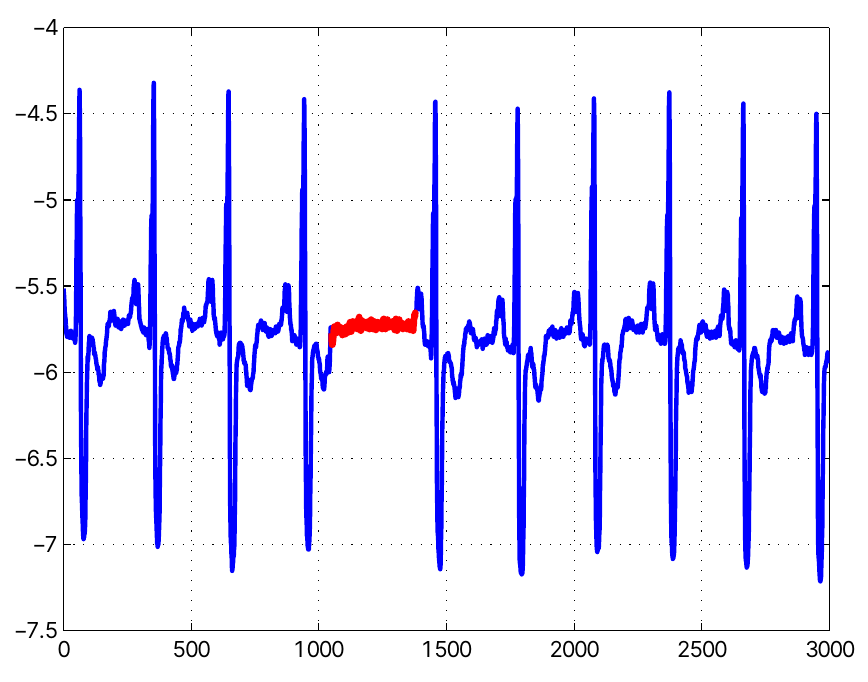
\includegraphics[width=0.4\paperwidth]{apc_ecg.png}}
	\caption{ Collective anomaly corresponding to an Atrial Premature Contraction in an human electrocardiogram output \cite{Goldberger2000PhysioBankPA} \cite{chandola2009anomaly}}
	\label{fig:apc_ecg}
\end{figure}


\subsection{Data labels}

The information associated with a data instance, describing if that instance is normal or anomalous is called label. Obtaining accurate and representative labeled data is often prohibitive expensive: it usually requires manual human effort, covering all possible scenarios of "anomalies" is expensive

Availability of labels influence the modality of the applicable anomaly detection techniques:

\subsubsection{Supervised}

In presence of training data with labeled data for both normal and anomaly class, this problem is similar to building predictive models for normal vs. anomaly classes.

Two issues can arise: \textit{imbalanced class distribution} and the non-triviliaty of \textit{obtaining accurate and significant labels} (especially for the anomaly class).


\subsubsection{Semi-supervised}

If training data has labeled instances for the normal class only, we resort to techniques operating in a semi-supervised mode, since they don't require labels for the anomaly class. The idea is to build a model for the normal behavior(s) and then use it to identify anomalous instances.

\subsubsection{Unsupervised}

This class includes the most widely applicable techniques, since they do not require any training data. Here, we assume that normal instances are more frequent than the anomalous ones. If this doesn't happen, an high false alarm rate is to be expected.


\subsubsection{Evaluation}

Here, we introduce some classification performance metrics used to set up a formal procedure to evaluate different approaches.

\begin{table}[]
	\centering
	\begin{tabular}{lllll}
		                                     &          &                                           &          & \\
		\multirow{2}{*}{}                    &          & \multicolumn{2}{l}{\textbf{Ground Truth}} &            \\
		                                     &          & Positive                                  & Negative & \\
		\multirow{2}{*}{\textbf{Prediction}} & Positive & TP                                        & FP       & \\
		                                     & Negative & FN                                        & TN       &
	\end{tabular}
	\caption{Confusion Matrix}
	\label{table:confusion_matrix}
\end{table}

Table \ref{table:confusion_matrix} explains the following quantities:

\begin{itemize}
	\item TP True Positives
	\item FP False Positives
	\item FN False Negatives
	\item TN True Negatives
\end{itemize}

Receiver Operating Characteristics (ROC) diagrams show a classifier performance plotting the False Positive Rates (FPR) against the True Positive Rates (TPR) of the classifier for a different thresholds. The idea is maximise the area under the ROC curve.

Intuitively, precision is the ability of the classifier not to label as positive a sample that is negative while recall is a measure of the ability of the classifier to find all the positive samples. \cite{scikit-learn}


\begin{equation}
	TPR = Recall = r = \frac{TP}{TP+FN}
\end{equation}

\begin{equation}
	FPR = \frac{FP}{FP+TN}
\end{equation}

\begin{equation}
	Precision = p = \frac{TP}{TP+FP}
\end{equation}

\begin{equation}
	Accuracy = \frac{TP+TN}{TP+TN+FP+FN}
\end{equation}

\begin{equation}
	Error = 1 - Accuracy
\end{equation}

Another metric is the F-measure, defined as follows:

\begin{equation}
	F_\beta = (1 + \beta^2) \cdot \frac{\mathrm{p} \cdot \mathrm{r}}{(\beta^2 \cdot \mathrm{p}) + \mathrm{r}}
\end{equation}

Where $\beta$ is a positive real chosen such that recall is considered $\beta$ times as important as precision. In the case $\beta = 1$, we have the $F_1$ score:

\begin{equation}
	F_1 = 2 \cdot \frac{\mathrm{p} \cdot \mathrm{r}}{\mathrm{p} + \mathrm{r}}
\end{equation}



\subsection{Output of Anomaly Detection}

Anomalies are Outputs produced by anomaly detection techniques can be Scores or Labels.


\subsection{Applications}



\section{Machine Learning}

\subsection{Artificial Neural Networks}

\textit{Artificial Neural Networks} are mathematical models inspired by biological neural networks. They are composed of (layers of) connected neurons and characterized by processes changing their structure based on the flowing information during the \textit{learning} stage.

The first mention of this term is in McCulloch and Pitts' 1943 work \cite{McCulloch1943}, where they introduced a Threshold Logic Unit (or Linear Threshold Unit), able to implement simple boolean functions \ref{fig:TLU}.

\begin{figure}[H]
	\centering
	\begin{equation*}
		\begin{aligned}[c]
			TLU(\vec{x}) & = \phi \bigg( \sum_{i=1}^{n}{w_{i} \cdot x_{i}} \bigg) \\
			\phi(x)      & = x - \theta \geq 0
		\end{aligned}
		\quad
		\begin{aligned}[c]
			n      & = 2   \\
			\theta & = 1.5 \\
		\end{aligned}
		\quad
		\begin{aligned}[c]
			w_{1} & = 1.0 \\
			w_{2} & = 1.0
		\end{aligned}
	\end{equation*}
	\caption{Boolean logic AND implemented by a Threshold Logic Unit}
	\label{fig:TLU}
\end{figure}

\paragraph{Perceptron}

Rosenblatt introduced in 1958 the \textit{Perceptron}\cite{rosenblatt1958perceptron}, a linear binary classificator now considered the simplest feed-forward neural network.

It can be modeled as follows:

\begin{equation*}
	\begin{aligned}[c]
		f(\mathbf{x}) = \begin{cases}1 & \text{if }\ \mathbf{w} \cdot \mathbf{x} + b > 0,\\0 & \text{otherwise}\end{cases}
	\end{aligned}
\end{equation*}

\begin{equation*}
	\begin{aligned}[c]
		w = \begin{bmatrix}
			w_{1} & \cdots & w_{d} & b
		\end{bmatrix}
	\end{aligned}
	\quad
	\begin{aligned}[c]
		\vec{x} = \begin{bmatrix}
			x_{1}  \\
			\vdots \\
			x_{d}  \\
			1
		\end{bmatrix}
	\end{aligned}
\end{equation*}

\begin{figure}[H]
	\centering
	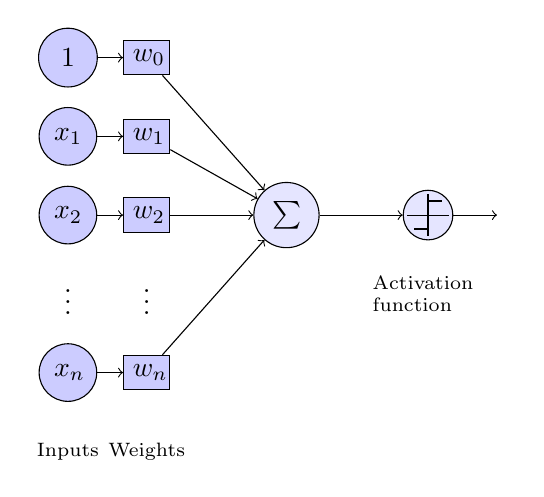
\begin{tikzpicture}
		\node[functions] (center) {};
		\node[below of=center,font=\scriptsize,text width=4em] {Activation function};
		\draw[thick] (0.5em,0.5em) -- (0,0.5em) -- (0,-0.5em) -- (-0.5em,-0.5em);
		\draw (0em,0.75em) -- (0em,-0.75em);
		\draw (0.75em,0em) -- (-0.75em,0em);
		\node[right of=center] (right) {};
		\path[draw,->] (center) -- (right);
		\node[functions,left=3em of center] (left) {$\sum$};
		\path[draw,->] (left) -- (center);
		\node[weights,left=3em of left] (2) {$w_2$} -- (2) node[input,left of=2] (l2) {$x_2$};
		\path[draw,->] (l2) -- (2);
		\path[draw,->] (2) -- (left);
		\node[below of=2] (dots) {$\vdots$} -- (dots) node[left of=dots] (ldots) {$\vdots$};
		\node[weights,below of=dots] (n) {$w_n$} -- (n) node[input,left of=n] (ln) {$x_n$};
		\path[draw,->] (ln) -- (n);
		\path[draw,->] (n) -- (left);
		\node[weights,above of=2] (1) {$w_1$} -- (1) node[input,left of=1] (l1) {$x_1$};
		\path[draw,->] (l1) -- (1);
		\path[draw,->] (1) -- (left);
		\node[weights,above of=1] (0) {$w_0$} -- (0) node[input,left of=0] (l0) {$1$};
		\path[draw,->] (l0) -- (0);
		\path[draw,->] (0) -- (left);
		\node[below of=ln,font=\scriptsize] {Inputs};
		\node[below of=n,font=\scriptsize] {Weights};
	\end{tikzpicture}
\end{figure}

\section{Activation Functions}

The choice of activation functions in neural networks affects the training dynamics and the final performance. A lot of alternatives have been proposed and are in development, but none managed to reach the popularity of ReLU.

\begin{description}[align=right,leftmargin=*,labelindent=5cm]
	\item[Sigmoid (Logistic)]
	      ${(1 + e^{-x})}^{-1}$
	\item[Hyperbolic]
	      $\tanh(x)$
	\item[Rectified Linear Unit (ReLU)]
	      $\max(0,\, x)$
	\item[Leaky ReLU]
	      $\max(0.01x,\, x)$
	\item[Parametric LReLU]
	      $\begin{cases}
			      \alpha x & \text{if } x \geq 0 \\
			      x        & \text{if } x < 0    \\
		      \end{cases}$
	\item[Exponential Linear Unit (ELU)]
	      $\begin{cases}
			      \alpha(e^x - 1) & \text{if } x \geq 0 \\
			      x               & \text{if } x < 0    \\
		      \end{cases}$
	\item[Swish]
	      $x \cdot \text{sigmoid}(\beta x)$
\end{description}

\begin{figure}
	\centerline{
		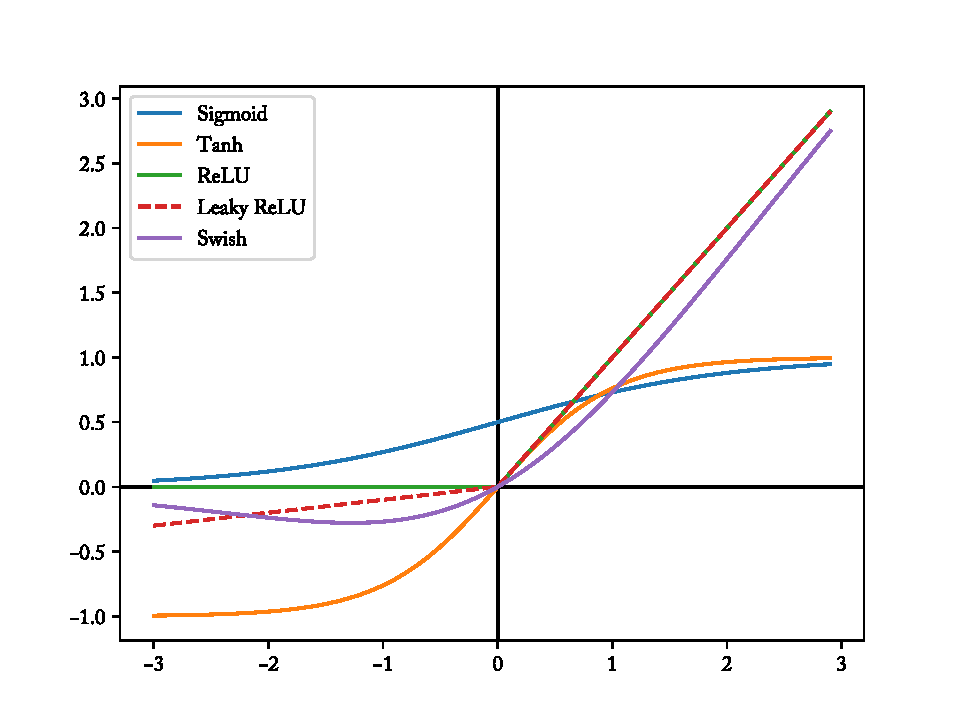
\includegraphics[width=0.7\paperwidth]{activation_fun_comparison}}
	\caption{Comparison of activation functions}
	\label{fig:activation_functions}
\end{figure}

Some important trends have been discovered by \textit{Searching for Activation Functions} \cite{DBLP:journals/corr/abs-1710-05941}, a recent study using automated search and benchmarking techniques:

\begin{enumerate}
	\item Complicated activation functions consistently underperform simpler activation functions;
	\item A common structure shared by the top activation functions is the use of the raw preactivation $x$ as input to the final binary function;
	\item Functions that use division tend to perform poorly because the output explodes when the denominator approaches zero.
\end{enumerate}

\section{Loss Functions}

\subsection{Regression loss}

\begin{equation}
	L_2(y, \hat{y}) = MSE = \sum\limits_{i=1}^n  {(y_i - \hat{y}_i)}^2
\end{equation}

\begin{equation}
	L_1(y, \hat{y}) = MAE = \sum\limits_{i=1}^n  {|y_i - \hat{y}_i|}
\end{equation}

\begin{equation}
	L_{cosh}(y, \hat{y}) = \sum\limits_{i=1}^n  {\log(\cosh(\hat{y}_i-y_i))}
\end{equation}

\begin{equation}
	L_\gamma(y, \hat{y}) = \sum\limits_{i=y_i<\hat{y}_i}  ({\gamma-1}).|y_i - \hat{y}_i| + \sum\limits_{i=y_i\geq \hat{y}_i}  ({\gamma}).|y_i - \hat{y}_i|
\end{equation}



\begin{figure}
	\centerline{
		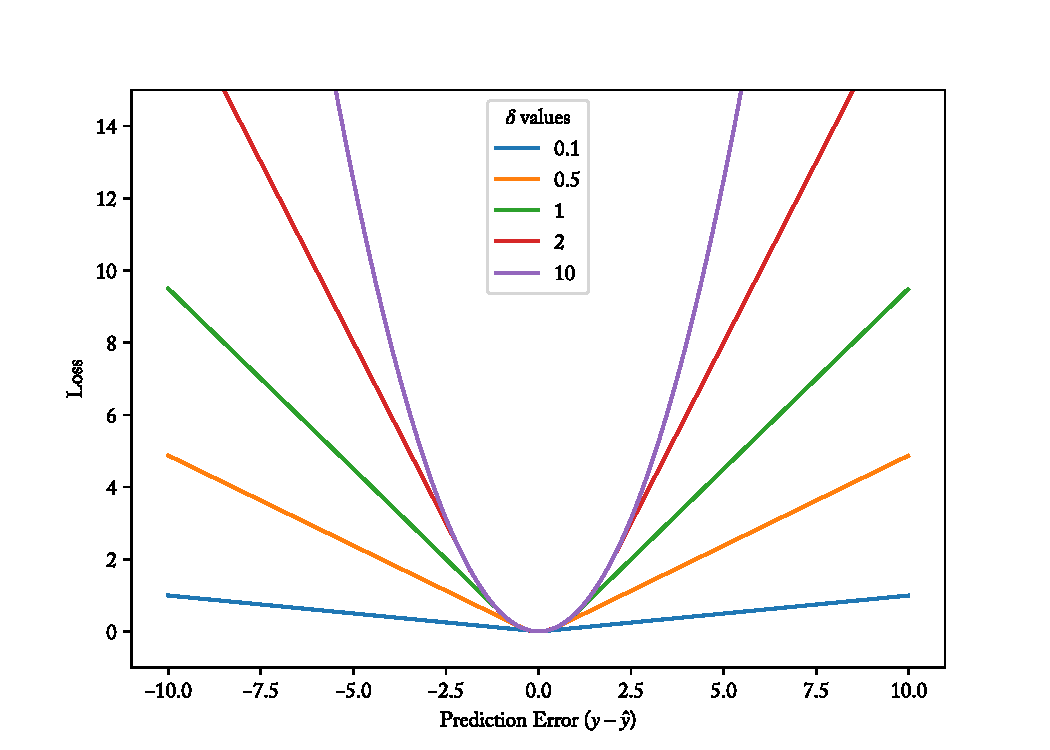
\includegraphics[width=0.6\paperwidth]{loss_Huber}}
	\caption{Huber/Smooth MAE Loss Function using various $\delta$ values}
	\label{fig:Loss Huber}
\end{figure}

\begin{figure}
	\centerline{
		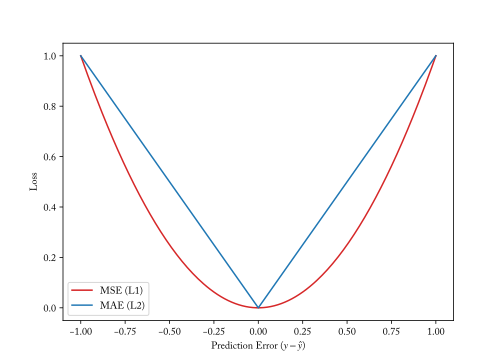
\includegraphics[width=0.6\paperwidth]{loss_L1_L2}}
	\caption{Mean Square Error (L2) vs Mean Absolute Error (L1) Loss Functions}
	\label{fig:Loss L1 L2}
\end{figure}

\begin{figure}
	\centerline{
		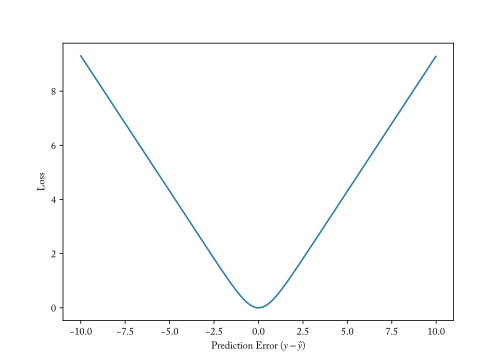
\includegraphics[width=0.6\paperwidth]{loss_logcosh}}
	\caption{Log-Cosh Loss Function}
	\label{fig:Loss L1 L2}
\end{figure}

\begin{figure}
	\centerline{
		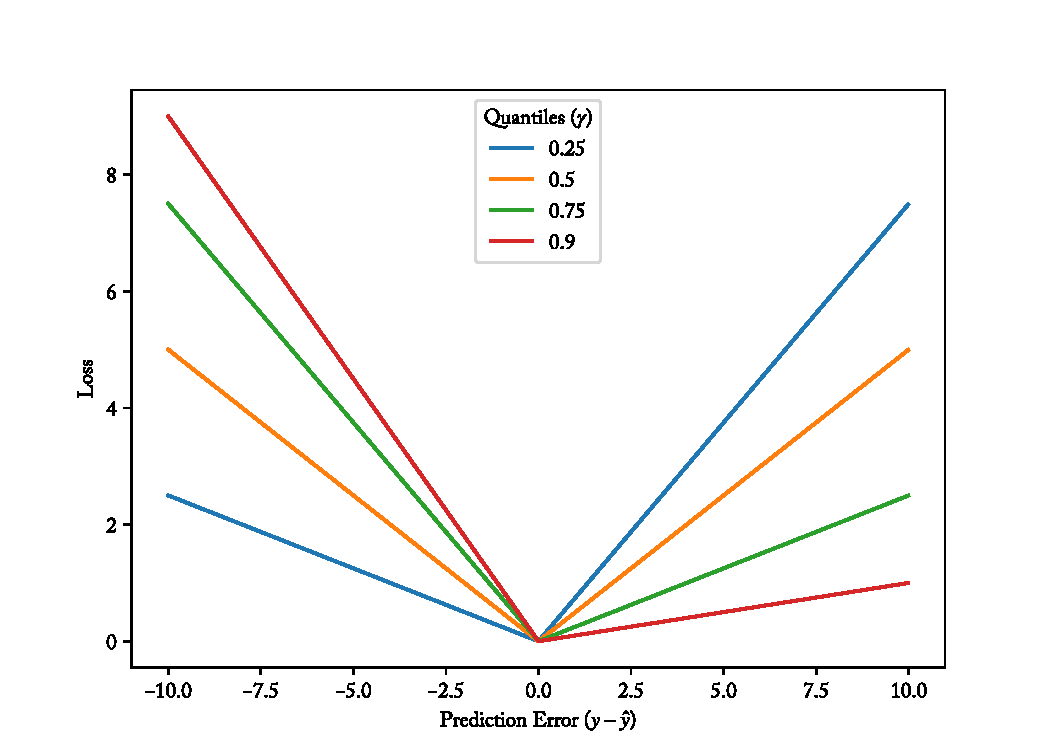
\includegraphics[width=0.6\paperwidth]{loss_quant}}
	\caption{Quantile Loss Function, with different Quantiles ($\gamma$) values}
	\label{fig:Loss L1 L2}
\end{figure}

\subsection{Classification loss}
\chapter{Modernising Rate Monitoring Tools}

One of the major challenges for the Compact Muon Solenoid (CMS) experiment, is the task of reducing event rate from roughly 40 MHz down to a more manageable 1 kHz while keeping as many interesting physics events as possible. This is accomplished through the use of a Level-1 (L1) hardware based trigger as well as a software based High-Level Trigger (HLT). Monitoring and understanding the output rates of the L1 and HLT triggers is of key importance for determining the overall performance of the trigger system and is intimately tied to what type of data is being recorded for physics analyses.

Here, we introduce the Trigger System in operation at the CMS experiment and proceed giving an overview of the software development work done to improve and add new features to the CMS Rate Monitoring software, a collection of tools used by CMS shifters to monitor the L1 and HLT trigger rates. Some other experimental components have ben developed to showcase possible upgrades, delivering quality of life enhancements and enabling shifters and physicists to navigate data in a faster and more comfortable way.

Finally, proper export functionalities have been added to the tools, allowing to save and export Trigger Rates as JSON or ROOT binary files.

This work is also described in \cite{VivaceRTM1} \cite{VivaceRTM2} \cite{L1TriggerOMSDevelopments} \cite{MohrmanRTM}, the source code is available in the RateMon git repository \cite{RateMonGit}.

\section{CMS Trigger System}

A Trigger is an  electronic system for spotting potentially interesting collisions in a particle detector and triggering the detector’s read-out system to record the data resulting from the collision.

The LHC generates 40 millions events per second. Each CMS event, on average, carries a payload of 1 MB of unprocessed informations. It is technologically impossible to retain this amount of data, due to hardware, software, network and storage constraints. Furthermore, most events represent uninteresting information for the current state of physics knowledge.

The \textit{CMS Trigger System} is designed to reduce the output stream to 1000 events per second, while preserving the physics reach of the experiment.
It is composed by a hierarchical set of rules, called Trigger Nodes (or Paths): each one probes a specific patterns (physics signature) in the event or looks for specific physics objects.

This happens in two steps:

\begin{enumerate}

    \item The first level (L1) \cite{Bayatyan:706847} brings the 40 MHz to a 100 kHz rate. Here, N Trigger Algorithms are implemented on custom electronics (FPGAs and ASICs) exploiting informations from sub-detector components.

    \item A configurable set of L1 Trigger Nodes seeds Triggers in the second level (HLT), implemented in software. The event stream is further refined, selecting an average rate of 400 Hz for offline event storage and certification \cite{Khachatryan_2017}. HLT runs 600 of these independent Trigger Paths.

\end{enumerate}

\begin{figure}
    \centerline{
        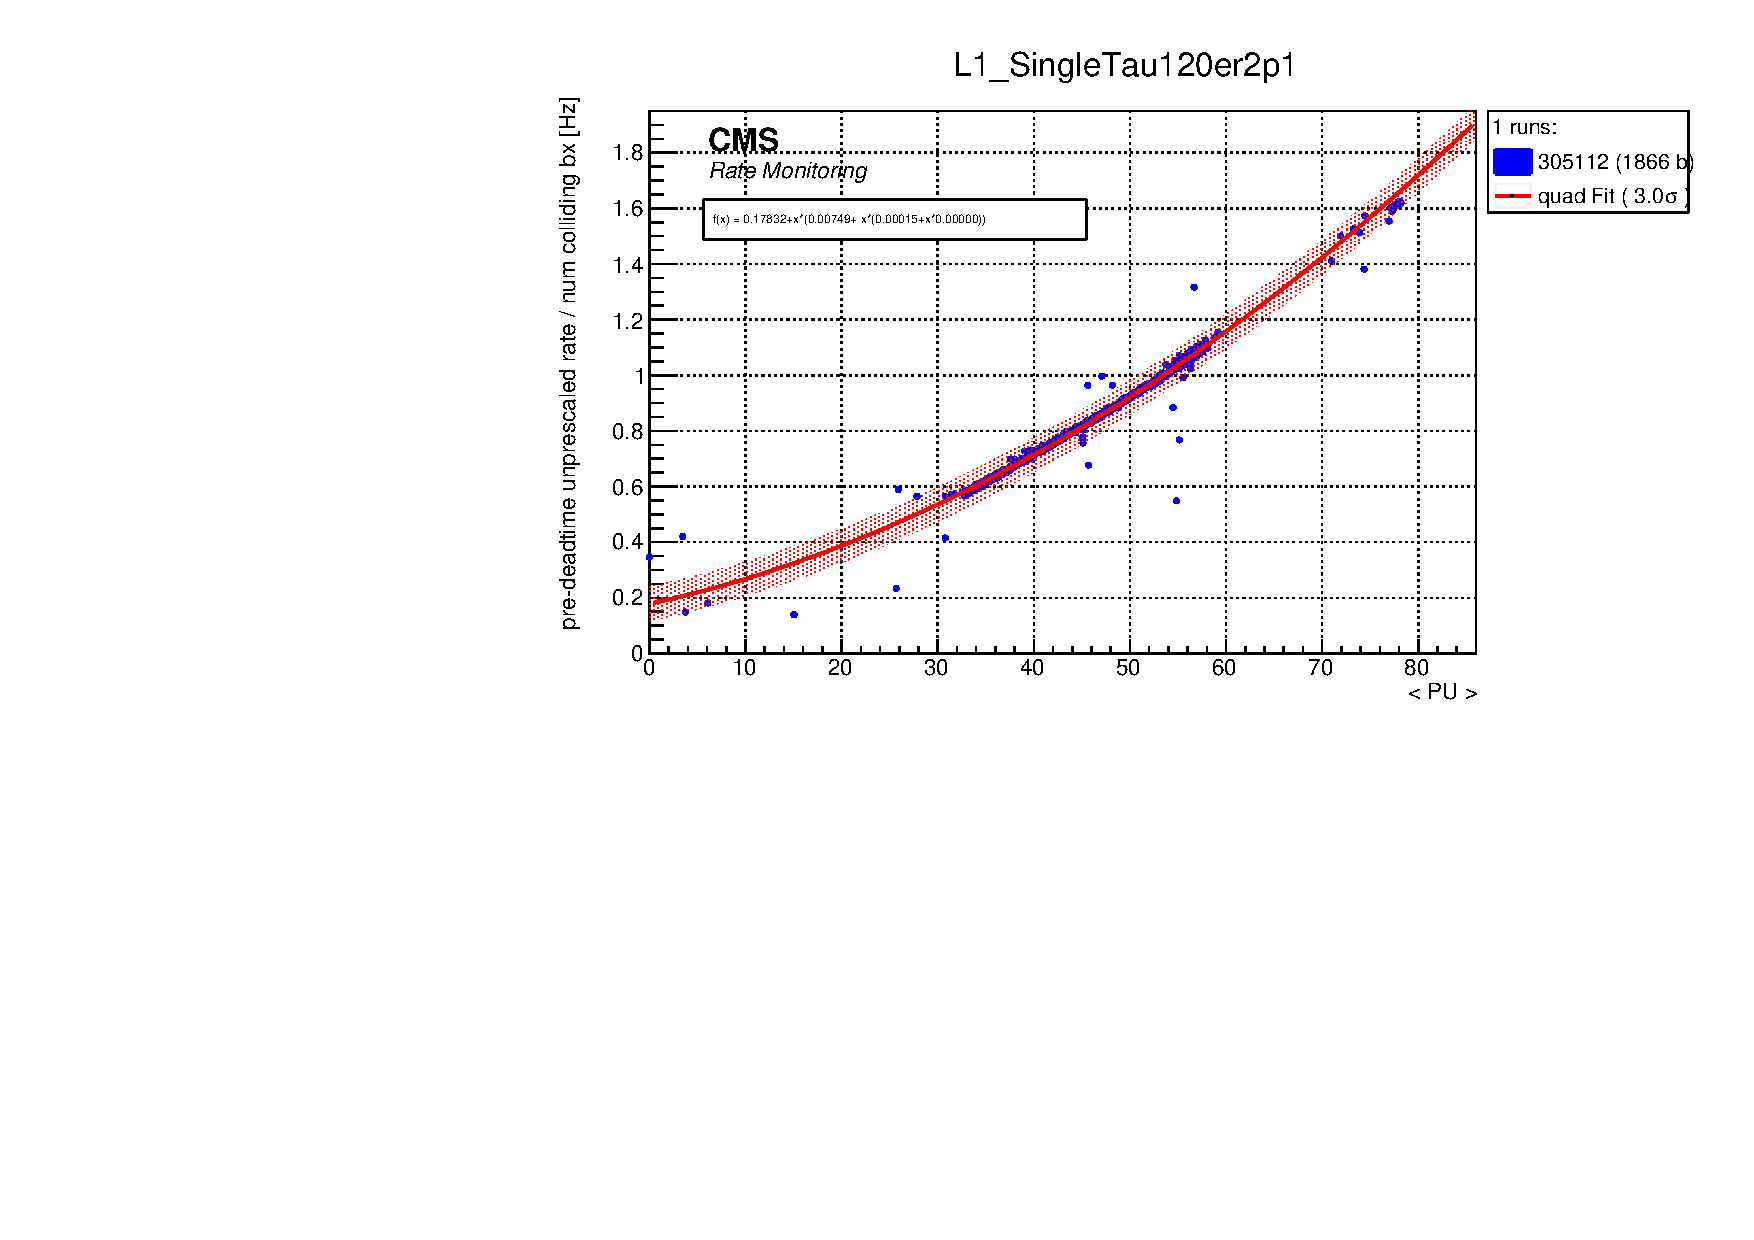
\includegraphics[width=0.6\paperwidth]{figures/RMT_305112_L1_SingleTau120er2p1.pdf}}
    \caption{L1 Trigger path plotted with a fitted function on run 305112}
    \label{fig:ratemon_l1}
\end{figure}

\begin{figure}
    \centerline{
        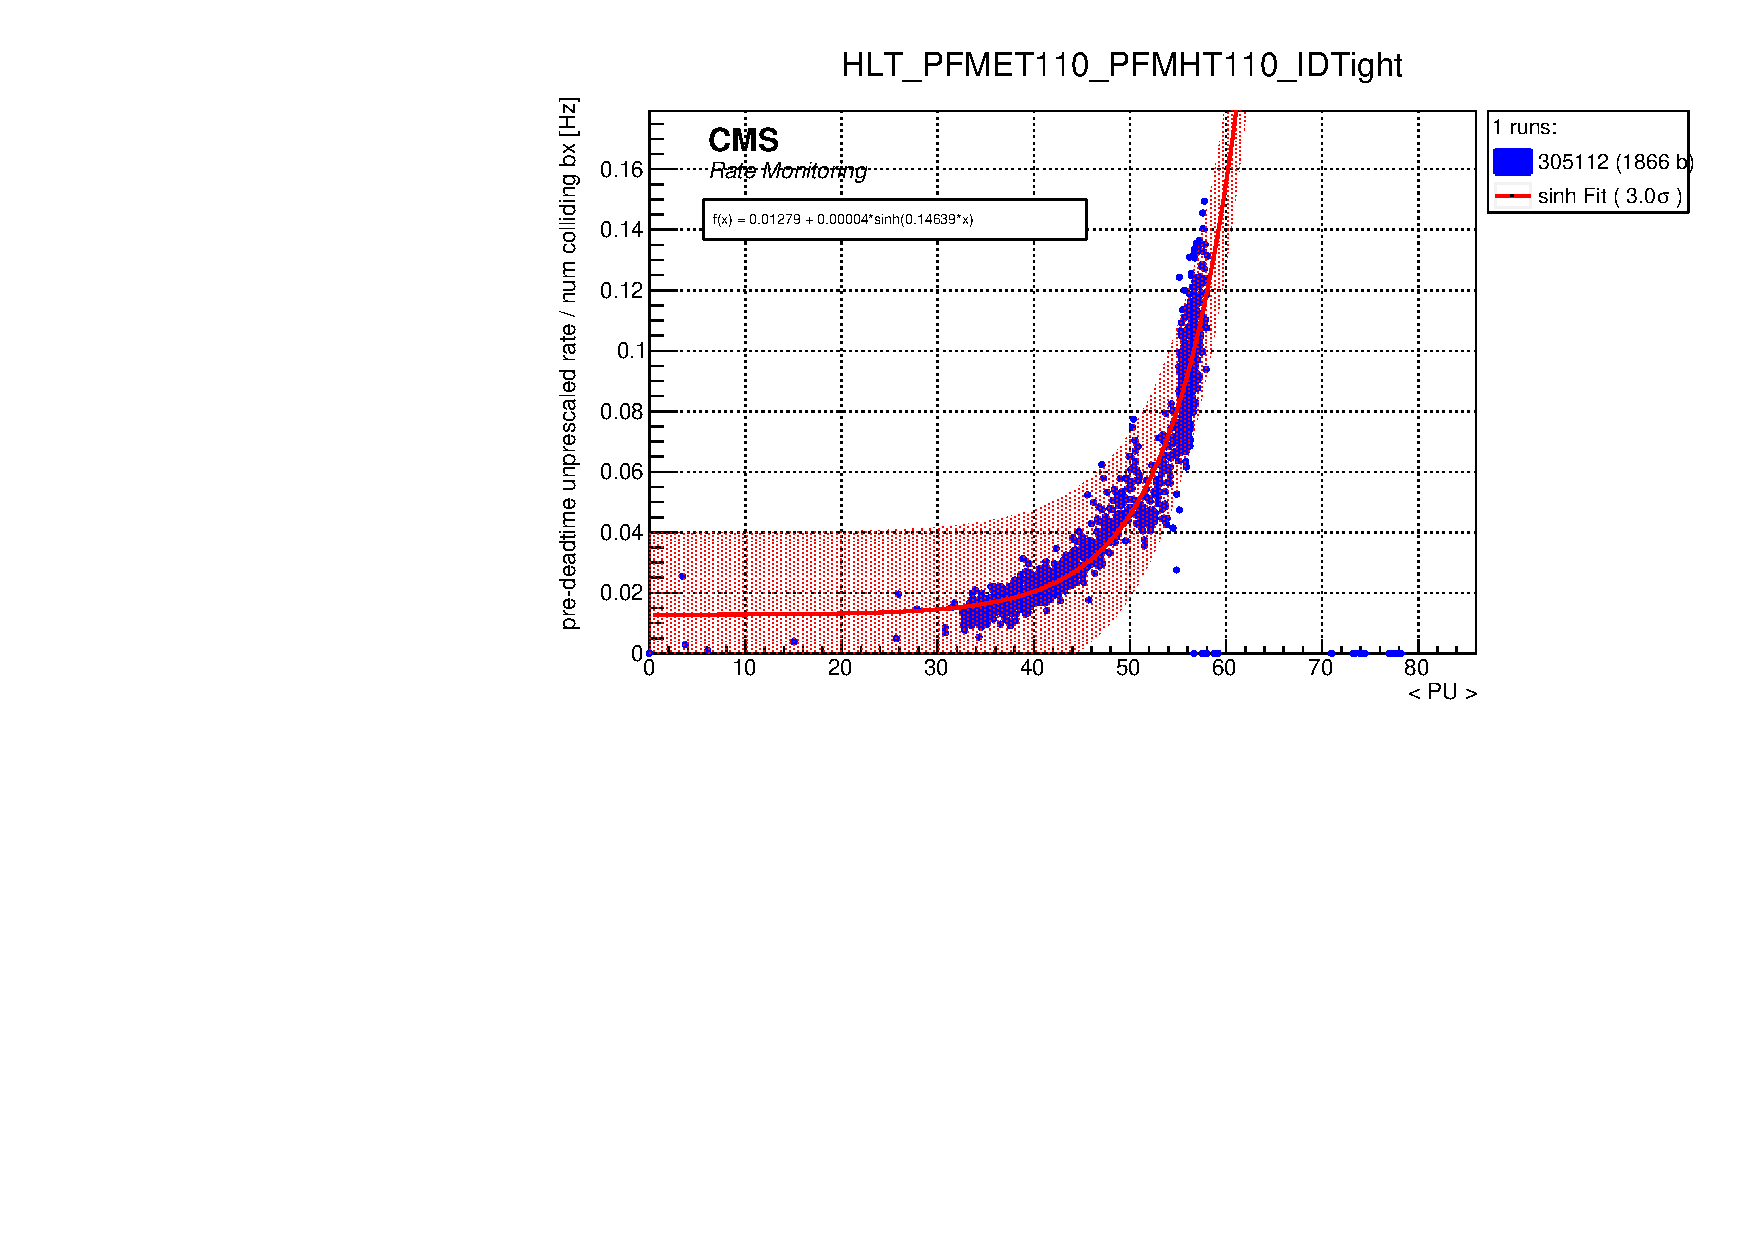
\includegraphics[width=0.6\paperwidth]{figures/RMT_305112_HLT_PFMET110_PFMHT110_IDTight.pdf}}
    \caption{HLT Trigger path plotted with a fitted function on run 305112}
    \label{fig:ratemon_hlt}
\end{figure}

\section{Rate Monitoring software}

\subsection{Shift Monitor tool}

The High Level Trigger (HLT) rate monitoring tool is a python script that reports the rates of a selected list of triggers, primary datasets, and streams. It is run in the CMS control room and gives valuable real-time feedback of trigger rates to the shift crew: it updates every minute and averages the rates recorded in the last 3 lumisections, and, if possible, compares them to the predicted rate. If a trigger path deviates by a specified amount from the prediction, or exceeds a fixed rate, the corresponding line is highlighted in a yellow colour. The scripts also displays other information that could be useful for the shifter, such as the run number and last lumisections, the LHC status, HLT key, deadtime, instantaneous luminosity and index of the prescale column in use.

\begin{figure}
    \centerline{
        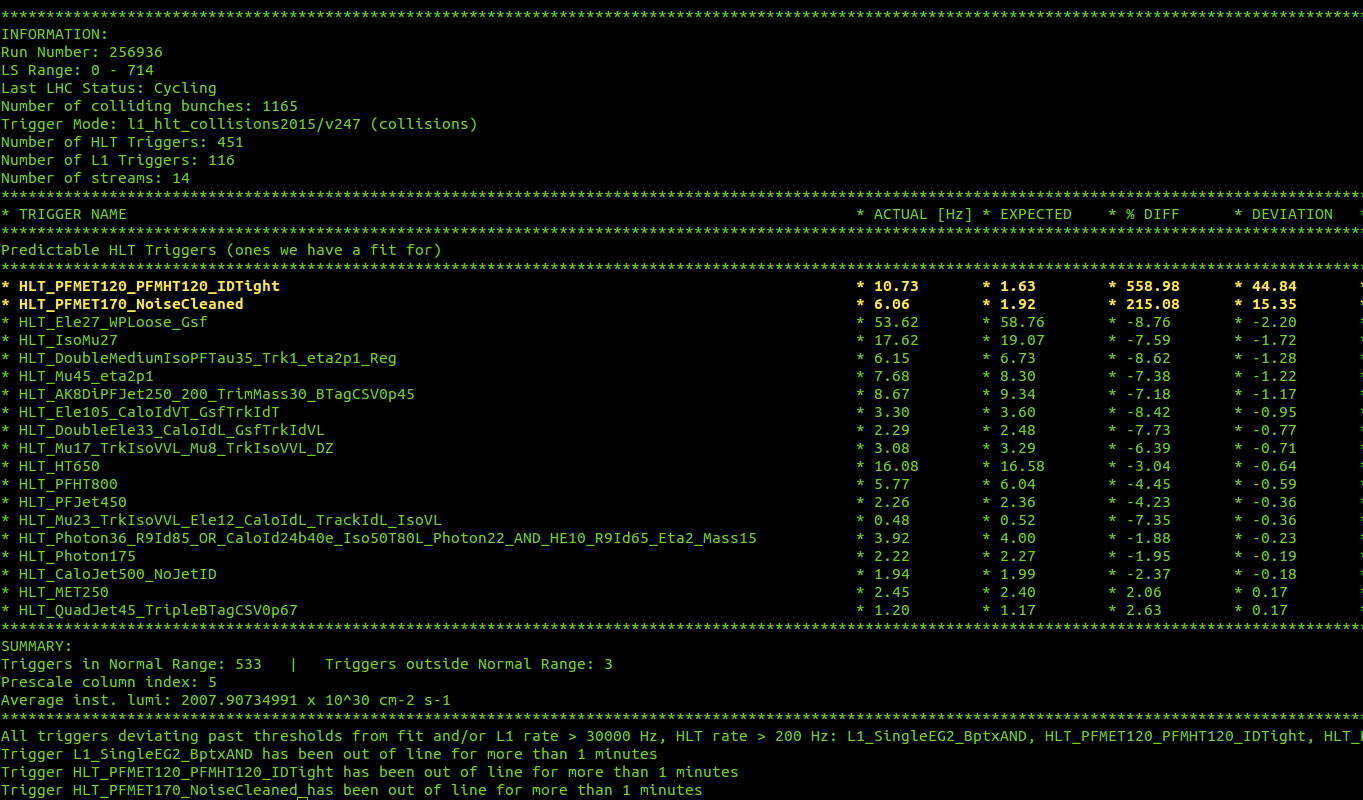
\includegraphics[width=0.8\paperwidth]{figures/ratemon_warnings}}
    \caption{Example execution of the Rate Monitoring Tool showing warnings: two triggers have values consistently deviating from the predictions. \cite{ratemon-twiki}}
    \label{fig:ratemon_warnings}
\end{figure}

\subsection{Trigger Rate plotting}

Another part of the software is plotting library, exposed as a the \texttt{plotTriggerRates} command line tool: it is used for observing how trigger rates vary over a range of beam and detector conditions, in particular how the rates of individual triggers scale with event pile-up.

Trigger Rates are usually represented in \textit{Rate vs. PileUp plots}, specifically "pre-deadtime unprescaled rate / num colliding bx [Hz]" over "PU" (Pile Up luminosity) units, generated by the RateMon tools.

In general, \textit{deadtime} refers to a time period during normal data taking when collisions are occurring but CMS is not ready to record the the data. This can occur for various reasons that are described in section 6.2.1 of \cite{Khachatryan_2017}. "pre-deadtime" rates are used in plots to allow for consistent comparison between different runs/fills; different runs and fills could have had different deadtimes, so correcting the rates for deadtime before fitting will allow the rates from different runs to be compared in a consistent way.

A \textit{prescale} is a way of scaling back the rate of L1 and HLT triggers. For example, if a certain trigger has a prescale of 5, then the data corresponding to the event the trigger fired on is only recorded once out of every five times that the trigger fired. So if the prescale is 1, the data will be recorded every time the trigger fires. A prescale of 0 actually means that no data will be recorded for the trigger in question; the trigger is essentially just turned off. Again, correcting for deadtime in Rate VS PU plots is to allow for consistent comparisons of rates for different runs/fills and across pre scale columns. 

\section{Packaging, CI/CD}

To enable CI/CD, we moved the repository on the CERN GitLab. The repository on GitHub is being kept updated but the CI/CD is handled by GitLab.
I've restructured the folder. The "misc" folder now contains the fits logs and the wbmRateReader. The ratemon folder is the only one actually being packaged. The "systemd" folder contains the service file allowing the \texttt{ShiftMonitorTool} to be installed and used as a systemd service.

Docker, GitLab ci, cernbox

Each commit triggers a build and a deployment of a RPM package. This CI/CD system is configured in these files:

\begin{enumerate}
    \item \texttt{.GitLab-ci.yml} describes the GitLab CI. The first phase (\texttt{build\_rpm}) tells the builder (described by \texttt{builder.dockerfile} and exposed on the GitLab registry) to run \texttt{make rpm} (described in \texttt{Makefile}) and flags the RPM package files as artifacts; In the second phase (deploy), those artifacts are pushed on a EOS folder using the ci-web-deployer tool;
    \item \texttt{builder.dockerfile} prepares the docker container that will run the build, starting from the cern/cc7-base image. This is exposed using the GitLab registry feature as \texttt{gitlab-registry.cern.ch/avivace/ratemon/builder};
    \item \texttt{Makefile} Uses the fpm tool to produce an RPM file with the given metadata and contents. Basically, the ratemon script folder is copied into /opt/ and the systemd service file goes into /usr/lib/systemd/system
    \item The build produces an RPM package file. Those files are pushed during the "deploy" CI phase and finally published on a public CERNBox folder (EOS: \texttt{/eos/users/a/avivace/ratemon\_builds}). This is done using a service CERN account.
\end{enumerate}

Previously, the RateMon tools had to be installed checking out the code from the git repository, running a preparatory script, configuring the database connection and then running the script. Now, the system package manager can install the packaged software.

\subsection{CMS Cactus}

TODO \cite{DirkxCactus}

\section{Configuration}

YAML, schema, database errors?

The ShiftMonitorTool and plotTriggerRates scripts now require an \texttt{--dbConfigFile} option, specifying the YAML configuration file containing the database connection parameters.

I've updated the README and the twiki page to reflect the changes on the DB configuration. Scripts now need to be called in this way:

\begin{textcode}
$ python plotTriggerRates.py --dbConfigFile=dbConfig.yaml --useFills --createFit --bestFit --triggerList=TriggerLists/monitorlistCOLLISIONS.list 6303
\end{textcode}

\section{Exporting data}

TODO

\subsection{Raw JSON}

TODO

\subsection{ROOT files}

TODO

\section{Python3 upgrade}

TODO

\section{From a CLI tool to a proper module}

\begin{listing}[ht]
\begin{pythoncode}
# Exporting trigger rates importing the plotTriggerRates class
import plotTriggerRates as ptr
import yaml

# Read database configuration from file
with open("dbConfig.yaml", 'r') as stream:
    dbCfg = yaml.safe_load(stream)

# Specify which triggers we want
triggers = ["HLT_Ele40_WPTight_Gsf",
              "HLT_DoubleEle33_CaloIdL_MW"]

# Initialize the RateMon controller
controller = ptr.MonitorController()

# Get Trigger Rates from Fill 6303, creating fits
triggerrates = controller.runStandalone(
                         dbConfig=dbCfg,
                         triggerList=triggers,
                         useFills=True,
                         vsLS=False,
                         createFit=True,
                         bestFit=True,
                         data_lst=[6303])

# Print result
print(triggerrates)
\end{pythoncode}
\caption{Example usage of the RateMon module in a Python script}
\end{listing}

\section{API}

\begin{figure}
    \centerline{
        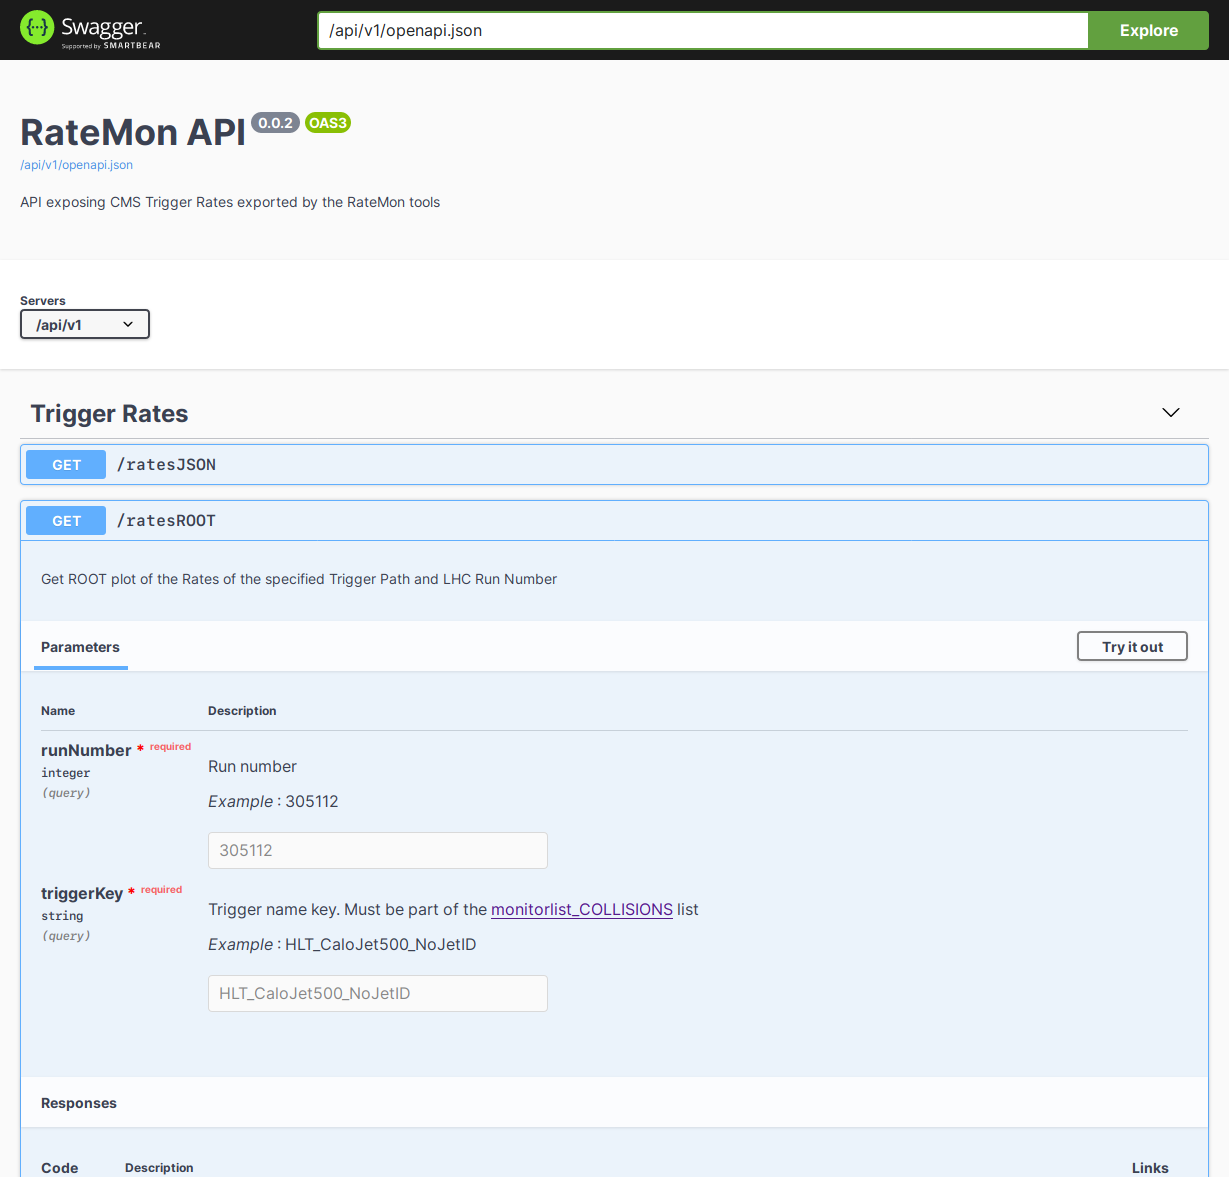
\includegraphics[width=0.8\paperwidth]{figures/swagger-ui}}
    \caption{Swagger UI}
    \label{fig:swagger-ui}
\end{figure}

\subsection{OpenAPI 3 Schema}

\begin{listing}[ht]
\begin{yamlcode}
openapi: "3.0.0"
info:
  version: 0.0.2
  title: RateMon API
  description: API exposing CMS Trigger Rates exported by the RateMon tools
servers:
  - url: http://ater.cern.ch/api/v1
paths:
  /ratesROOT:
    get:
      tags: [Trigger Rates]
      description: |
        Get ROOT plot of the Rates of the specified Trigger Path and LHC Run Number
      operationId: app.getRatesROOT
      parameters:
        - name: runNumber
          in: query
          description: "Run number"
          example: 305112
          required: true
          style: form
          schema:
            type: integer
        - name: triggerKey
          in: query
          description: "Trigger name key. Must be part of the [monitorlist_COLLISIONS](https://gitlab.cern.ch/cms-tsg-fog/ratemon/-/blob/api/ratemon/TriggerLists/monitorlist_COLLISIONS.list) list"
          example: HLT_CaloJet500_NoJetID
          required: true
          schema:
            type: string
      responses:
        '200':
          description: ROOT binary file of the computed plot
\end{yamlcode}
\caption{OpenAPI schema definition of the \texttt{/ratesROOT} API endpoint}
\end{listing}

Connexion, OpenAPI 3 schema, Swagger UI

\subsection{Implementation}

\begin{listing}[ht]
\begin{pythoncode}
def getRatesROOT(runNumber: int, triggerKey: str):
    saveDirectory = "/rtmdata/" + str(runNumber)
    rates = controller.runStandalone(
                         dbConfig=dbCfg,
                         exportRoot=True,
                         saveDirectory=saveDirectory,
                         makeTitle=False,
                         triggerList=[triggerKey],
                         createFit=True,
                         bestFit=True,
                         data_lst=[runNumber])

    return send_from_directory(saveDirectory,
                               triggerKey + '.ROOT',
                               as_attachment=True) # Keep the filename
\end{pythoncode}
\caption{Implementation of the \texttt{/ratesROOT} API endpoint}
\end{listing}

\subsection{Running}
\begin{textcode}
yum install libnsl

export LD_LIBRARY_PATH=/usr/lib/oracle/19.6/client64/lib:LD_LIBRARY_PATH

copy tnsnames.ora

wget https://download.oracle.com/otn_software/linux/instantclient/19600/oracle-instantclient19.6-basic-19.6.0.0.0-1.x86_64.rpm

yum install oracle-instantclient19.6-basic-19.6.0.0.0-1.x86_64.rpm
\end{textcode}

\section{Integration with OMS}

Highcharts, React, Panel

\section{Run Registry}

CMS Run Registry is a in-development tool giving access to a lot of DQM datasets. TODO: describe bug reports, HTTPS auth problems and various contributions done upstream to this tool.


\section{Deployment}

\subsection{Attaching a volume for caching}

To offer more disk space to the caching mechanism, a new volume has been created through the CERN Openstack control panel. Once available, I attached it to the machine serving the RateMon API.

On that machine, \texttt{fdisk -l} will give the disks overview, listing the new volume. I noted the device ID (\texttt{/dev/vdb}) and then executed \texttt{fdisk /dev/vdb} to launch fdisk, the partition manager tool provided by the util-linux standard package.

\begin{textcode}
$ fdisk -l
...
Disk /dev/vdb: 600 GiB, 644245094400 bytes, 1258291200 sectors
Units: sectors of 1 * 512 = 512 bytes
Sector size (logical/physical): 512 bytes / 512 bytes
I/O size (minimum/optimal): 512 bytes / 512 bytes
\end{textcode}

In the fdisk shell, create a new partition (\texttt{n}), select is a primary (\texttt{p}) and denote it as the first (\texttt{1}). Set it to occupy all the available space accepting defaults. Select again the partition (\texttt{t}) and set the Linux partition type (\texttt{83}). (\texttt{p}) displays the partition setup we just defined. If that's okay, (\texttt{w}) commits the modifications and applies them.

\begin{textcode}
Device     Boot Start        End    Sectors  Size Id Type
/dev/vdb1        2048 1258291199 1258289152  600G 83 Linux
\end{textcode}

Back in the standard shell, use \texttt{mkfs.ext4 /dev/vdb} to format the partition using the EXT4 file system.

Note the UUID of our newly formatted partition:

\begin{textcode}
$ mkfs.ext4 /dev/vdb
mke2fs 1.45.4 (23-Sep-2019)
Creating filesystem with 157286400 4k blocks and 39321600 inodes
Filesystem UUID: f74a87c8-7ced-4414-bc62-e09d07be7845
\end{textcode}

Now that we know the UUID, we can mount the volume:

\begin{textcode}
$ mkdir /cache
$ mount /dev/disk/by-uuid/f74a87c8-7ced-4414-bc62-e09d07be7845 /cache
\end{textcode}

To make the mounting persistent, we add this entry to the \texttt{/etc/fstab} file:

\begin{textcode}
UUID=f74a87c8-7ced-4414-bc62-e09d07be7845   /cache  auto defaults,nofail    0 3
\end{textcode}

Here's the final situation, as described by \texttt{df -h}:

\begin{textcode}
$ df -h
Filesystem      Size  Used Avail Use% Mounted on
...
/dev/vda2        40G   33G  7.6G  82% /
/dev/vdb        590G   73M  560G   1% /cache
\end{textcode}

\subsection{NGINX as reverse proxy and cache server}


\begin{textcode}
sudo cat /var/log/audit/audit.log | grep nginx | grep denied
\end{textcode}


\begin{textcode}
$ setsebool -P httpd_can_network_connect 1
\end{textcode}

chown nginx:nginx /cache/

\begin{listing}[ht]
\begin{nginxcode}
# Set cache dir
proxy_cache_path /cache levels=1:2 keys_zone=one:50m max_size=500g inactive=200d;

# Set cache key to include identifying components
proxy_cache_key $scheme$proxy_host$request_uri;

# Add cache status to log
log_format cache '$remote_addr - $remote_user [$time_local] "$request" $status $body_bytes_sent "$http_referer" "$http_user_agent" cs=$upstream_cache_status';

server {
    server_name ater.cern.ch;
    add_header X-Cache-Status $upstream_cache_status;
    
    ## Access and error logs.
    access_log /var/log/nginx/api-proxy.access.log cache;
    error_log  /var/log/nginx/api-cache.error.log;  
    
    location / {
        proxy_set_header Host $host;
        proxy_set_header X-Real-IP $remote_addr;
            
        proxy_cache one;
        proxy_ignore_headers X-Accel-Expires Expires Cache-Control;
        proxy_cache_valid 200 302 200d;
        proxy_cache_valid 404 15m;
        proxy_pass http://localhost:8085;   
    
    }
    listen 80;
}
\end{nginxcode}
\caption{NGINX configuration for reverse proxying and caching}
\end{listing}

\section{A new User Interface}

VueJS, ROOT, Plotly, Plotly -> JSROOT

\begin{figure}
    \centerline{
        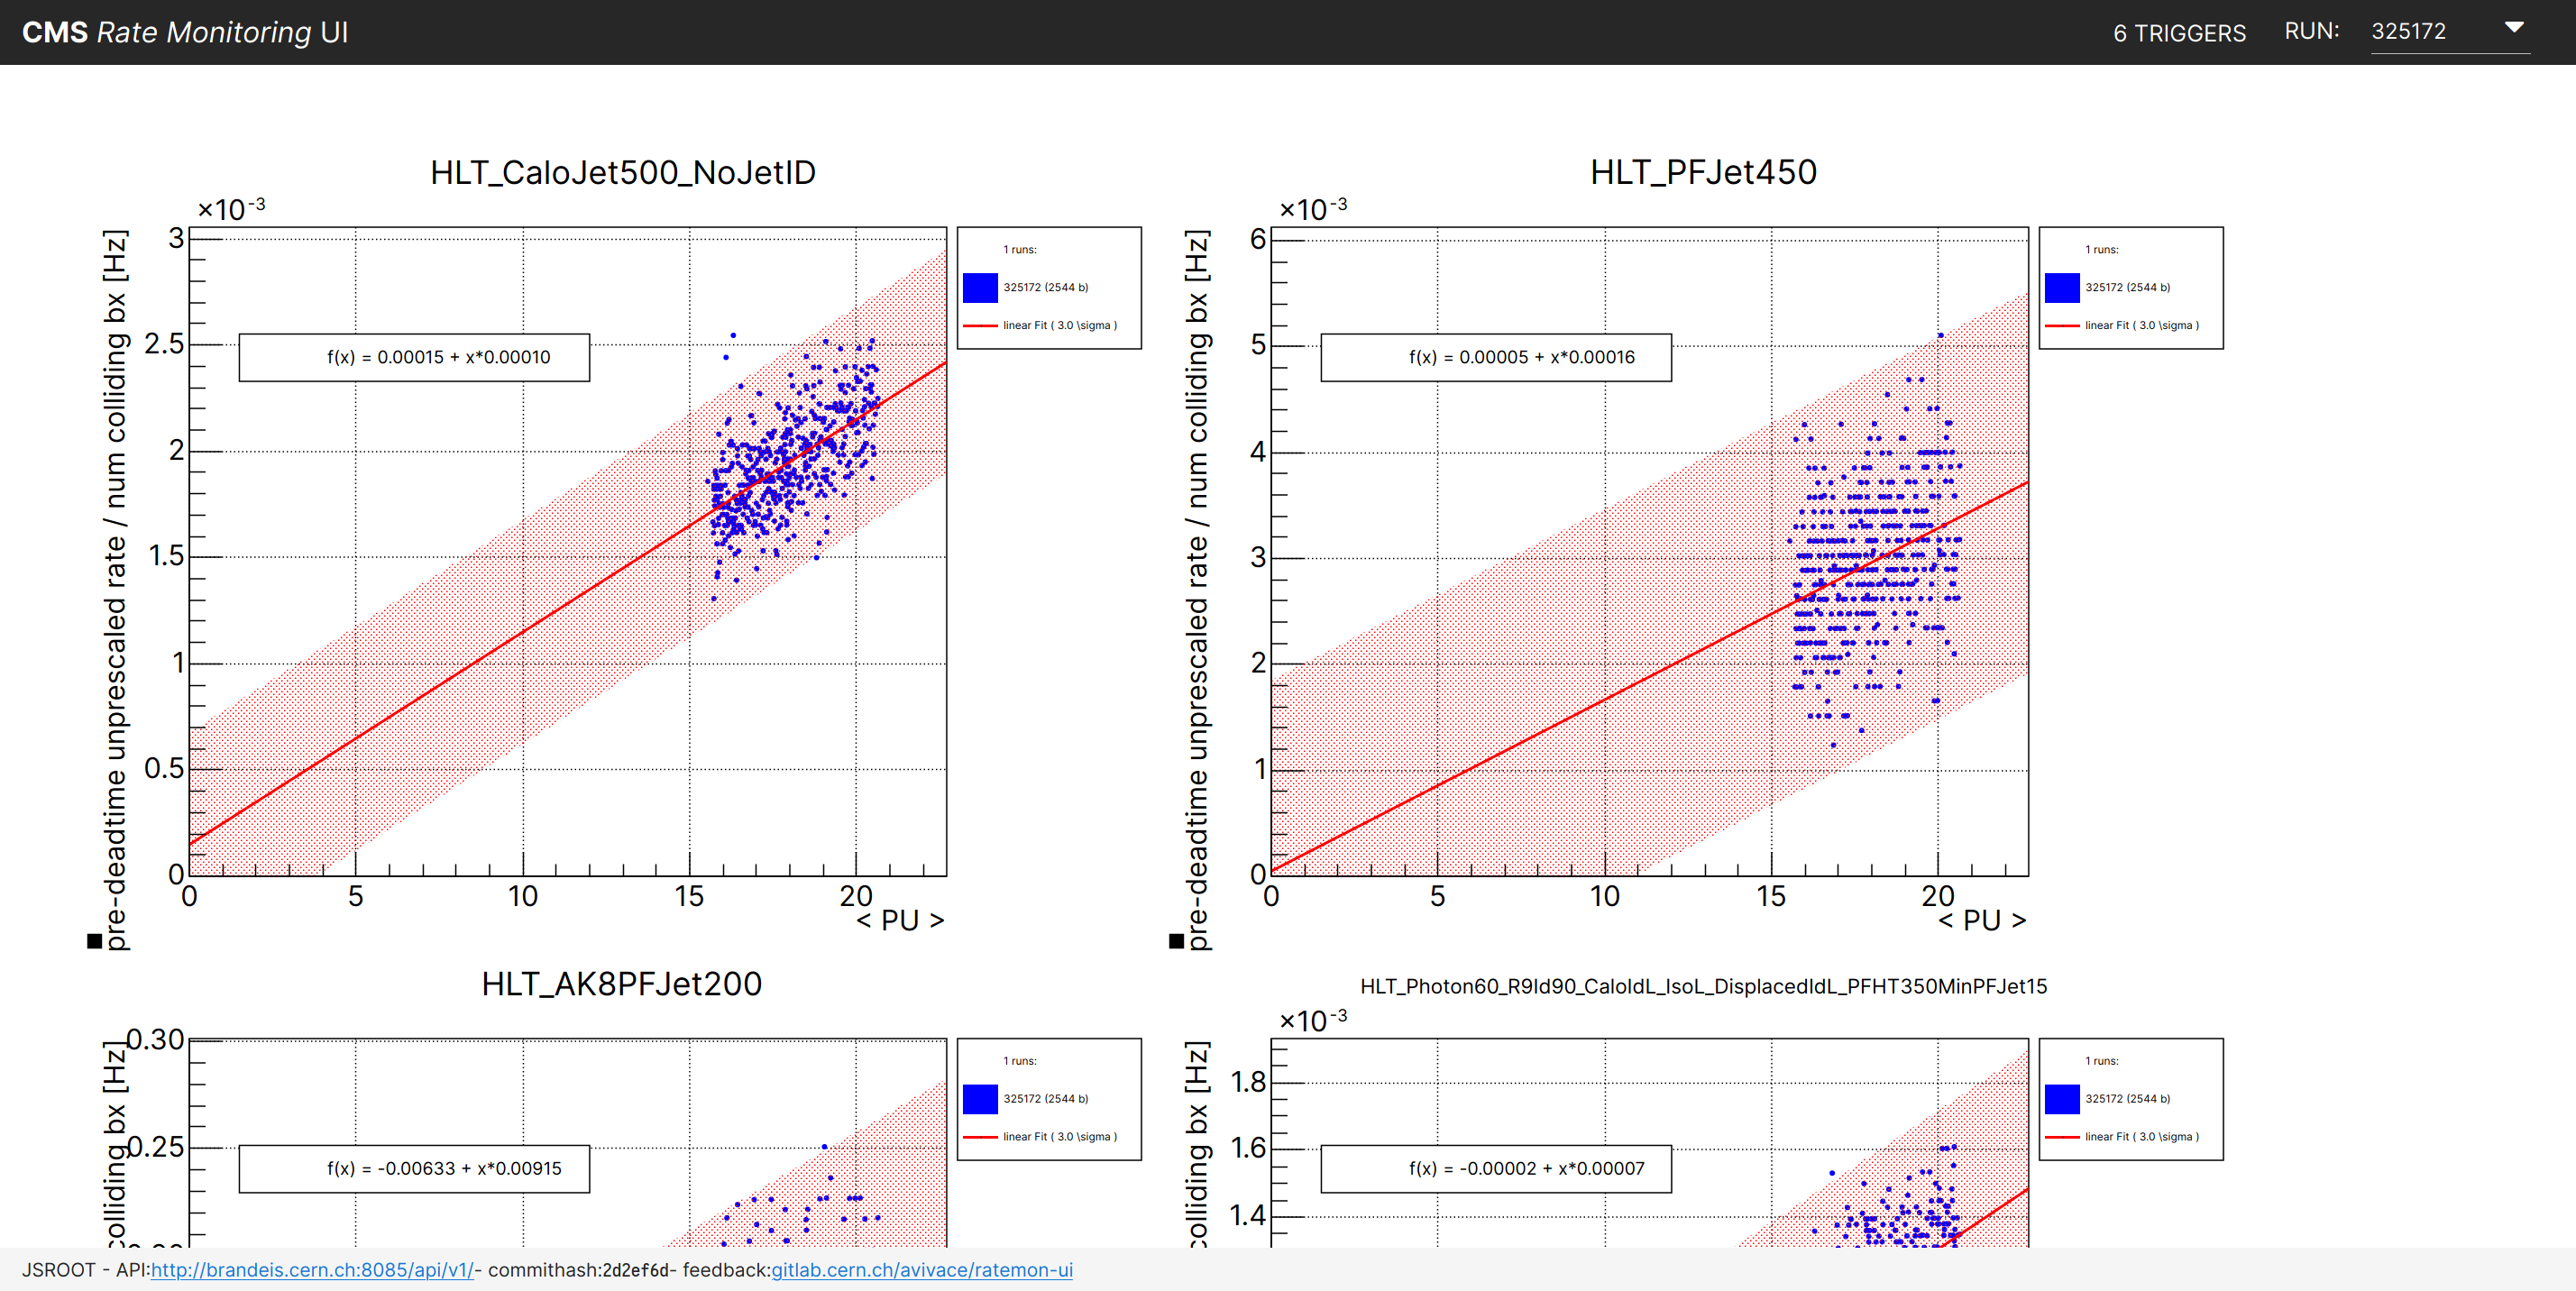
\includegraphics[width=0.9\paperwidth]{figures/ratemon-ui0.png}}
    \caption{Main RateMon UI application view, showing interactive trigger rate plots and relative fit functions}
    \label{fig:ratemon_ui0}
\end{figure}

\chapter{Anomaly Detection on Trigger Rates}
\label{dataset}
\section{Problem Statement}

\section{Data}

\subsection{Dataset A: Detector state over time}

This dataset describes the status of the CMS detector and its sub-systems over the progress of the Run, for every Run since the experiment is active.

The time progress of the Run is expressed in LS (Lumi Sections) units (\ref{ls_def}).

More than 25 thousands Run are available, starting from the 2009 collisions to the 2018 cosmics.

It's been generated using the CMS Run Registry API, with the DQM Offline Datasets as source.

\begin{listing}[H]
\begin{jsoncode}
  {
    "class": "Collisions18",
    "dataset_attributes": {},
    "datasets_in_gui": [],
    "deleted": false,
    "lumisections": {
      "btag-btag": {
        "EMPTY": 0,
        "GOOD": 228,
        "causes": [
          "UNDEF"
        ],
        "comments": []
      },
      "csc-csc": {
        "EMPTY": 0,
        "GOOD": 228,
        "causes": [
          "UNDEF"
        ],
        "comments": []
      },
      "dt-dt": {
        "EMPTY": 0,
        "GOOD": 228,
        "causes": [
          "UNDEF"
        ],
        "comments": []
      },
      "tracker-tracking": {
        "EMPTY": 0,
        "GOOD": 228,
        "causes": [
          "UNDEF"
        ],
        "comments": []
      },
      /* ... */
    },
    "name": "online",
    "run_number": 316361,
    "short_run": 1,
    "significant": true,
    "state": "SIGNOFF",
    "stop_reason": "ECAL preshower red recycle",
    "version": 4260755
  }
\end{jsoncode}
\caption{JSON export of the Run Registry data for Run 316361}
\end{listing}

\subsection{Dataset B: Trigger Rates}

For each Run we then exported the Trigger Rates in the form of "pre-deadtime unprescaled rate / num colliding bx" (Hz) values over LS time series.

There are hundreds of Triggers available, we selected the ones normally considered by shifters during Collision runs, which includes 17 HLT and 12 L1 Trigger Paths.

This data is generated querying data from the CMS OMDS database by the Rate Monitoring tools, which operates a series of normalisations to make the plots comparable across runs and configurations. A fitted function is also computed and included in the object describing the rates.

\begin{listing}[H]
\begin{jsoncode}
{
    "runnumber": 316361,
    "x_axis": "ls",
    "y_axis": "pre-dt-unprescaled-rate",
    "plots": {
        "HLT_DoubleEle33_CaloIdL_MW": {
            "plotname": "HLT_DoubleEle33_CaloIdL_MW_lumisection_vs_pre-deadtime unprescaled rate",
            "xvar": "lumisection",
            "yvar": "pre-deadtime unprescaled rate",
            "xVals": [
                23.0,
                24.0,
                25.0,
                // ...
            ],
            "yVals": [
                0.0038020953070372343,
                0.00429236376658082,
                0.005365777760744095,
                // ...
            ],
            "fit": {
                "linear": "0.00448 + x*-0.00000"
            }
        }
        // ...
    }
}

\end{jsoncode}
\caption{JSON export of Trigger Rates vs LS time series for Run 316361}
\end{listing}

\section{Anomaly Detection Pipeline}

\section{Results}

% Glossary
\glsaddall
\printglossaries

% List of Figures
\pagebreak
\listoffigures

% List of Listings
\pagebreak
\listoflistings
\addcontentsline{toc}{chapter}{List of Listings}

% References
\printbibheading[title={References}]
\printbibliography[nottype=online, heading=subbibliography, title=Bibliography]
\printbibliography[type=online, heading=subbibliography, title=Sitography]

% License
\pagebreak
\thispagestyle{empty}
\noindent
\copyright 2019 -- 2020 Antonio Vivace. This work is licensed under a Creative Commons Attribution-ShareAlike 4.0 International License.

\end{document}